\section{Optical Flow: Đo lường Chuyển động trong Video}
\label{sec:optical_flow}

\subsection{Giới thiệu: Khi Thế giới bắt đầu Chuyển động}
\label{subsec:optical_flow_intro}

Cho đến nay, toàn bộ hành trình của chúng ta trong Chương 2 đã tập trung vào các \textit{bức ảnh tĩnh}. Chúng ta đã học cách lọc, phát hiện cạnh, trích xuất các điểm đặc trưng, và xây dựng các bộ mô tả như SIFT hay HOG—tất cả đều hoạt động trên một khung hình đơn lẻ, đông cứng trong thời gian. Nhưng thế giới thực không phải là một bức tranh đóng khung trên tường. Nó chuyển động, thở, và thay đổi liên tục.

Một chiếc xe đang lăn bánh, một bàn tay đang vẫy chào, dòng nước chảy qua những tảng đá—tất cả đều là những tín hiệu thị giác không thể nắm bắt bằng một khung hình duy nhất. Để "nhìn" được những chuyển động này, máy tính cần một công cụ mới: khả năng đo lường sự di chuyển của các điểm ảnh từ khung hình này sang khung hình tiếp theo.

Công cụ đó có tên là \textbf{Optical Flow (Luồng quang học)}.

\begin{mdframed}[style=infobox]
    \textbf{Định nghĩa}

    Optical flow là trường vector 2D biểu diễn sự dịch chuyển biểu kiến (apparent motion) của mỗi pixel từ khung hình $I_t$ sang khung hình $I_{t+1}$. Tại mỗi pixel $(x, y)$, vector $(u, v)$ mô tả nó đã di chuyển bao nhiêu pixel theo chiều ngang ($u$) và chiều dọc ($v$).
\end{mdframed}

\begin{center}
    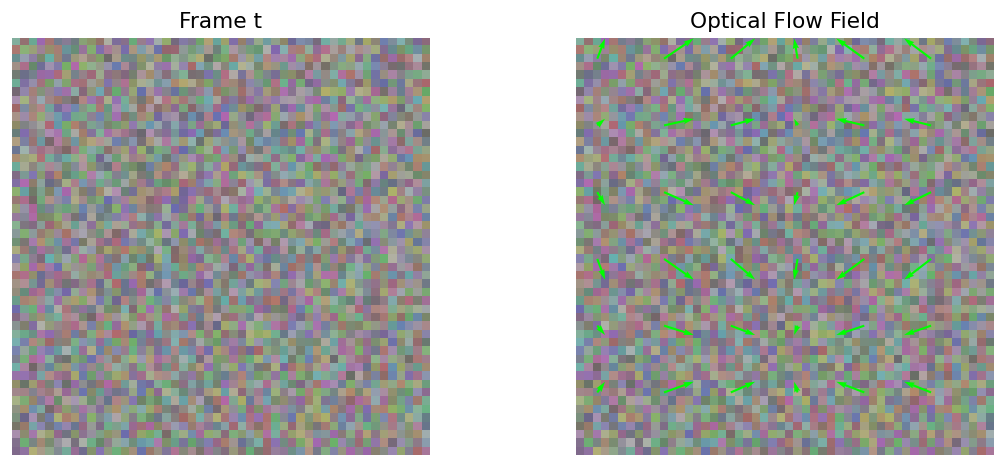
\includegraphics[width=0.85\textwidth]{images/optical_flow_example.png}
    \captionof{figure}{Minh họa Optical Flow. (Trái) Hai khung hình liên tiếp của một video người đang di chuyển. (Phải) Trường optical flow tương ứng, được biểu diễn bằng các mũi tên màu. Hướng và độ dài của mỗi mũi tên cho biết hướng và tốc độ di chuyển của pixel tương ứng.}
    \label{fig:optical_flow_example}
\end{center}

Optical flow có mặt ở khắp nơi trong các hệ thống thị giác máy tính hiện đại:
\begin{itemize}
    \item \textbf{Theo dõi đối tượng (Object Tracking):} Biết được luồng quang học cho phép dự đoán vị trí của một đối tượng trong khung hình tiếp theo.
    \item \textbf{Nhận dạng hành động (Action Recognition):} Chuyển động của tay, chân, và thân người mã hóa thông tin phân biệt hành động "chạy" với "đi bộ" hay "nhảy".
    \item \textbf{Nén video:} Các codec video hiện đại như H.264 sử dụng ý tưởng tương tự để chỉ lưu trữ \textit{sự thay đổi} giữa các khung hình, tiết kiệm dung lượng đáng kể.
    \item \textbf{Ổn định video (Video Stabilization):} Bù trừ chuyển động của camera để tạo ra video mượt mà.
    \item \textbf{Điều hướng robot và xe tự lái:} Ước tính chuyển động của bản thân (ego-motion) và phát hiện các vật cản đang di chuyển.
\end{itemize}

\subsection{Giả thiết Bất biến Độ sáng và Phương trình Optical Flow}
\label{subsec:brightness_constancy}

Mọi phương pháp tính optical flow đều dựa trên một giả thiết nền tảng, đơn giản nhưng mạnh mẽ:

\begin{mdframed}[style=infobox]
    \textbf{Giả thiết Bất biến Độ sáng (Brightness Constancy Assumption)}

    Cường độ sáng của một điểm trong cảnh vật không thay đổi khi nó di chuyển từ khung hình này sang khung hình tiếp theo.
    \[
        I(x, y, t) = I(x + u, y + v, t + 1)
    \]
    trong đó $(u, v)$ là vector dịch chuyển (optical flow) của pixel $(x, y)$.
\end{mdframed}

Dùng khai triển Taylor bậc nhất cho vế phải:
\[
    I(x + u, y + v, t + 1) \approx I(x, y, t) + \frac{\partial I}{\partial x}u + \frac{\partial I}{\partial y}v + \frac{\partial I}{\partial t}
\]

Kết hợp với giả thiết bất biến độ sáng ($I(x,y,t) = I(x+u,y+v,t+1)$), ta thu được \textbf{Phương trình Ràng buộc Optical Flow}:

\begin{equation}
    \frac{\partial I}{\partial x}u + \frac{\partial I}{\partial y}v + \frac{\partial I}{\partial t} = 0
    \label{eq:optical_flow_constraint}
\end{equation}

hay viết gọn hơn: $I_x u + I_y v + I_t = 0$, trong đó $I_x, I_y$ là gradient không gian của ảnh và $I_t$ là gradient thời gian (sự thay đổi cường độ giữa hai khung hình).

Đây là một phương trình với hai ẩn số $(u, v)$—bài toán thiếu ràng buộc (underdetermined). Chính đây là biểu hiện toán học của \textbf{vấn đề khẩu độ (aperture problem)} đã đề cập ở phần trước. Để giải được, mỗi phương pháp optical flow phải đưa ra thêm các giả thiết bổ sung.

\subsection{Lucas-Kanade: Optical Flow Cục bộ}
\label{subsec:lucas_kanade}

\subsubsection{Giả thiết Chuyển động Đồng nhất Cục bộ}
\label{subsubsec:lk_assumption}

Phương pháp Lucas-Kanade (1981) \cite{Lucas1981} giải quyết bài toán thiếu ràng buộc bằng một giả thiết rất tự nhiên: \textbf{tất cả các pixel trong một vùng lân cận nhỏ $\Omega$ (ví dụ: cửa sổ $5 \times 5$ hoặc $7 \times 7$) quanh pixel đang xét đều có cùng một vector optical flow $(u, v)$}.

Khi đó, phương trình ràng buộc được áp dụng cho mỗi pixel $(x_i, y_i)$ trong vùng lân cận $\Omega$:

\[
    \begin{pmatrix}
        I_x(x_1, y_1) & I_y(x_1, y_1) \\
        I_x(x_2, y_2) & I_y(x_2, y_2) \\
        \vdots & \vdots \\
        I_x(x_n, y_n) & I_y(x_n, y_n)
    \end{pmatrix}
    \begin{pmatrix} u \\ v \end{pmatrix}
    =
    -\begin{pmatrix}
        I_t(x_1, y_1) \\
        I_t(x_2, y_2) \\
        \vdots \\
        I_t(x_n, y_n)
    \end{pmatrix}
\]

hay dạng ma trận: $A\mathbf{d} = -\mathbf{b}$.

\subsubsection{Giải bằng Bình phương Tối tiểu}
\label{subsubsec:lk_least_squares}

Hệ phương trình trên là over-determined (nhiều phương trình hơn ẩn số), được giải bằng phương pháp bình phương tối tiểu (least squares):

\begin{equation}
    \begin{pmatrix} u \\ v \end{pmatrix}
    = (A^T W A)^{-1} A^T W (-\mathbf{b})
    \label{eq:lucas_kanade_solution}
\end{equation}

trong đó $W$ là ma trận trọng số Gaussian (nhấn mạnh các pixel ở trung tâm cửa sổ). Ma trận $A^T W A$ chính là \textbf{ma trận cấu trúc} quen thuộc từ phần Harris Corner Detector:

\[
    M = A^T W A = \begin{pmatrix} \sum w I_x^2 & \sum w I_x I_y \\ \sum w I_x I_y & \sum w I_y^2 \end{pmatrix}
\]

\begin{mdframed}[style=infobox]
    \textbf{Kết nối sâu sắc: Optical Flow và Corner Detection}

    Nhớ lại Harris Corner Detector: ma trận $M$ có cả hai trị riêng lớn tại các góc. Điều này có nghĩa là $(A^T W A)$ trong Lucas-Kanade sẽ khả nghịch tốt (well-conditioned) tại chính xác những vị trí là các góc! Đây là lý do tại sao Shi-Tomasi được gọi là "Good Features to Track"—chỉ những điểm góc mới có thể được theo dõi chính xác bằng Lucas-Kanade. Tại các điểm trên cạnh thẳng, vấn đề khẩu độ xuất hiện và $M$ trở nên suy biến.
\end{mdframed}

\subsubsection{Phiên bản Đa tỉ lệ (Pyramid Lucas-Kanade)}
\label{subsubsec:lk_pyramid}

Phương pháp Lucas-Kanade cơ bản chỉ hoạt động tốt với các chuyển động nhỏ (dưới 1-2 pixel). Để xử lý các chuyển động lớn hơn, người ta sử dụng kỹ thuật \textbf{kim tự tháp ảnh (image pyramid)}:

\begin{enumerate}
    \item Xây dựng kim tự tháp Gaussian gồm nhiều mức: mỗi mức có kích thước bằng một nửa mức trước đó.
    \item Tính optical flow thô tại mức đỉnh (ảnh nhỏ nhất, chuyển động lớn trở thành nhỏ).
    \item Lan truyền ước tính đó xuống mức dưới và tinh chỉnh dần.
\end{enumerate}

Phương pháp này giải quyết được các chuyển động lớn một cách hiệu quả và là cơ sở của hàm \texttt{cv2.calcOpticalFlowPyrLK} trong OpenCV.

\begin{minted}[fontsize=\footnotesize, frame=single, linenos=true]{python}
import cv2
import numpy as np

cap = cv2.VideoCapture('video.mp4')

# Đọc khung hình đầu tiên
ret, prev_frame = cap.read()
prev_gray = cv2.cvtColor(prev_frame, cv2.COLOR_BGR2GRAY)

# Phát hiện các điểm đặc trưng tốt để theo dõi (Shi-Tomasi)
feature_params = dict(maxCorners=100, qualityLevel=0.3,
                      minDistance=7, blockSize=7)
p0 = cv2.goodFeaturesToTrack(prev_gray, mask=None, **feature_params)

# Tham số cho Lucas-Kanade pyramid
lk_params = dict(winSize=(15, 15), maxLevel=2,
                 criteria=(cv2.TERM_CRITERIA_EPS | cv2.TERM_CRITERIA_COUNT,
                           10, 0.03))

while True:
    ret, frame = cap.read()
    if not ret:
        break
    frame_gray = cv2.cvtColor(frame, cv2.COLOR_BGR2GRAY)

    # Tính optical flow: theo dõi p0 từ prev_gray sang frame_gray
    p1, st, err = cv2.calcOpticalFlowPyrLK(prev_gray, frame_gray,
                                            p0, None, **lk_params)
    # st=1: điểm được theo dõi thành công
    good_new = p1[st == 1]
    good_old = p0[st == 1]

    # Vẽ các vector chuyển động
    for new, old in zip(good_new, good_old):
        a, b = new.ravel().astype(int)
        c, d = old.ravel().astype(int)
        cv2.arrowedLine(frame, (c, d), (a, b), (0, 255, 0), 2)

    prev_gray = frame_gray.copy()
    p0 = good_new.reshape(-1, 1, 2)

cap.release()
\end{minted}

\subsection{Horn-Schunck: Optical Flow Toàn cục}
\label{subsec:horn_schunck}

Cùng năm 1981, Horn và Schunck \cite{HornSchunck1981} đề xuất một cách tiếp cận khác. Thay vì giả thiết chuyển động đồng nhất trong một cửa sổ nhỏ, họ đưa ra giả thiết \textbf{toàn cục}: optical flow phải \textit{mượt mà} trên toàn bộ ảnh (các pixel lân cận có xu hướng chuyển động giống nhau).

Bài toán được đặt ra dưới dạng tối thiểu hóa một hàm năng lượng:

\begin{equation}
    E(u, v) = \iint \underbrace{\left(I_x u + I_y v + I_t\right)^2}_{\text{data term}} + \lambda^2 \underbrace{\left(|\nabla u|^2 + |\nabla v|^2\right)}_{\text{smoothness term}} \, dx\, dy
    \label{eq:horn_schunck_energy}
\end{equation}

\begin{itemize}
    \item \textbf{Data term:} Phạt vi phạm phương trình ràng buộc optical flow.
    \item \textbf{Smoothness term:} Phạt sự thay đổi đột ngột của $(u, v)$ giữa các pixel lân cận.
    \item $\lambda$: Tham số cân bằng giữa hai số hạng.
\end{itemize}

So với Lucas-Kanade, Horn-Schunck tạo ra trường optical flow \textbf{dày đặc (dense)} và \textbf{mượt mà} hơn trên toàn bộ ảnh, nhưng đòi hỏi giải một hệ phương trình lớn và nhạy cảm hơn với nhiễu.

\subsection{Optical Flow Học sâu: FlowNet và RAFT}
\label{subsec:deep_optical_flow}

\subsubsection{Hạn chế của các Phương pháp Cổ điển}
\label{subsubsec:classical_of_limitations}

Lucas-Kanade và Horn-Schunck hoạt động tốt trong nhiều tình huống, nhưng đều dựa trên giả thiết bất biến độ sáng—một giả thiết dễ bị vi phạm khi ánh sáng thay đổi, có phản chiếu gương (specular reflection), hay vật thể quay. Chúng cũng gặp khó khăn với các chuyển động lớn và không đồng nhất.

Kể từ năm 2015, các phương pháp học sâu đã cách mạng hóa lĩnh vực này, tự động học cách ước tính optical flow từ hàng triệu cặp khung hình.

\subsubsection{FlowNet (2015): Kiến trúc Encoder-Decoder}
\label{subsubsec:flownet}

FlowNet \cite{Dosovitskiy2015} là mạng CNN đầu tiên học ước tính optical flow end-to-end. Kiến trúc của nó theo dạng encoder-decoder:

\begin{itemize}
    \item \textbf{Encoder:} Nhận đầu vào là hai khung hình đặt chồng thành 6 kênh, trích xuất đặc trưng qua các lớp tích chập giảm dần kích thước.
    \item \textbf{Decoder:} Giải mã đặc trưng trở lại độ phân giải gốc bằng các lớp deconvolution (transposed convolution), xuất ra trường optical flow dày đặc.
\end{itemize}

FlowNet đánh dấu bước ngoặt: lần đầu tiên một mạng học được cách "nhìn thấy chuyển động" một cách tự động.

\subsubsection{RAFT (2020): Trạng thái Nghệ thuật Hiện đại}
\label{subsubsec:raft}

RAFT (Recurrent All-Pairs Field Transforms) \cite{Teed2020} của Teed và Deng đã thiết lập trạng thái nghệ thuật hiện đại với một kiến trúc ba bước thanh lịch:

\begin{enumerate}
    \item \textbf{Feature Extraction:} Trích xuất đặc trưng từ cả hai khung hình bằng một mạng CNN dùng chung trọng số.
    \item \textbf{4D Correlation Volume:} Tính tích vô hướng (dot product) giữa \textit{mọi cặp} pixel từ hai khung hình, tạo ra một volume 4D $(H \times W \times H \times W)$ mô tả "mức độ tương tự" giữa mọi cặp vị trí.
    \item \textbf{Iterative Refinement (GRU):} Sử dụng một đơn vị hồi quy (GRU) để lặp đi lặp lại tinh chỉnh ước tính optical flow hiện tại bằng cách tra cứu correlation volume theo từng bước nhỏ.
\end{enumerate}

\begin{center}
    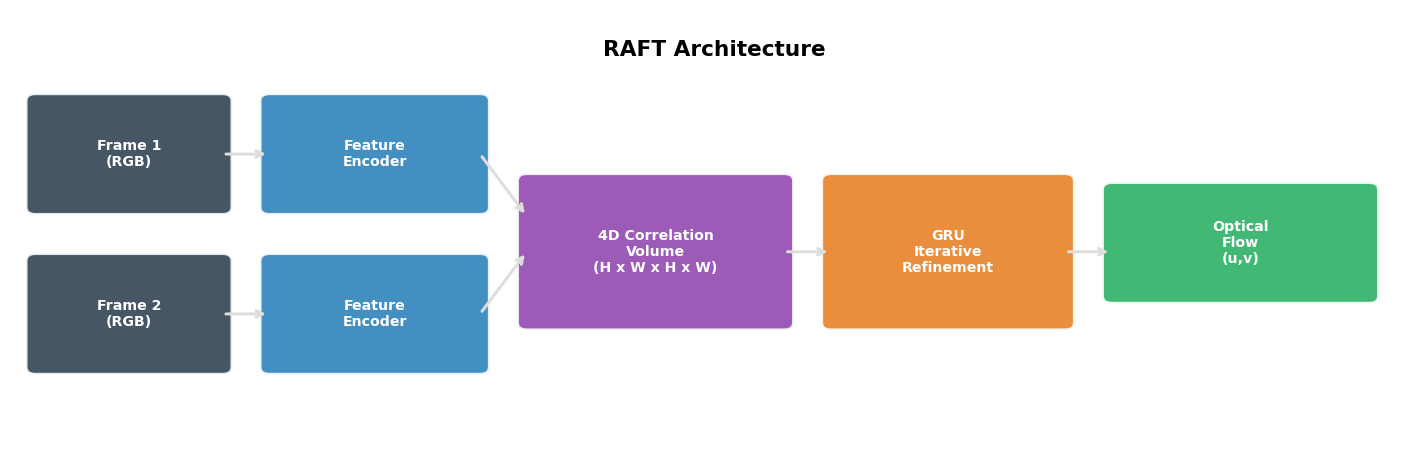
\includegraphics[width=0.9\textwidth]{images/raft_architecture.png}
    \captionof{figure}{Kiến trúc RAFT. Hai nhánh trích xuất đặc trưng song song, theo sau là tính toán correlation volume 4D và một module tinh chỉnh lặp (iterative refinement) dựa trên GRU. Phương pháp này đạt độ chính xác vượt trội so với các phương pháp trước đó.}
    \label{fig:raft_architecture}
\end{center}

RAFT vượt trội hơn tất cả các phương pháp trước đó trên benchmark Sintel và KITTI, và tư duy "iterative refinement" của nó đã trở thành chuẩn mực cho thế hệ mô hình tiếp theo.

\subsection{So sánh các Phương pháp}
\label{subsec:optical_flow_comparison}

\begin{table}[h!]
    \centering
    \caption{So sánh các phương pháp Optical Flow}
    \label{tab:optical_flow_comparison}
    \begin{tabular}{|l|p{3.5cm}|p{3.5cm}|p{3.5cm}|}
        \hline
        \textbf{Tiêu chí} & \textbf{Lucas-Kanade} & \textbf{Horn-Schunck} & \textbf{RAFT} \\
        \hline
        \textbf{Loại} & Sparse (tại keypoints) & Dense (toàn ảnh) & Dense (toàn ảnh) \\
        \hline
        \textbf{Giả thiết} & Cục bộ đồng nhất & Toàn cục mượt mà & Học từ dữ liệu \\
        \hline
        \textbf{Tốc độ} & Rất nhanh & Chậm (iterative) & Nhanh (GPU) \\
        \hline
        \textbf{Độ chính xác} & Tốt khi chuyển động nhỏ & Tốt, mượt mà & Tốt nhất hiện tại \\
        \hline
        \textbf{Robustness} & Thấp (nhạy ánh sáng) & Thấp & Cao \\
        \hline
        \textbf{Ứng dụng} & Tracking real-time & Phân tích chuyển động & Video understanding \\
        \hline
    \end{tabular}
\end{table}

Optical flow là cầu nối thiết yếu giữa thị giác trên ảnh tĩnh và thị giác trên video. Những khái niệm được xây dựng ở đây—từ giả thiết bất biến độ sáng cho đến RAFT—sẽ tái xuất hiện khi chúng ta thảo luận về Video Understanding ở các chương sau.

\section*{Tài liệu tham khảo}
\begin{itemize}
    \item[1] Lucas, B. D.; Kanade, T. An Iterative Image Registration Technique with an Application to Stereo Vision. In \textit{Proceedings of IJCAI}, 1981.
    \item[2] Horn, B. K. P.; Schunck, B. G. Determining Optical Flow. \textit{Artificial Intelligence} \textbf{1981}, \textit{17}(1-3), 185-203.
    \item[3] Dosovitskiy, A. et al. FlowNet: Learning Optical Flow with Convolutional Networks. In \textit{ICCV}, 2015.
    \item[4] Teed, Z.; Deng, J. RAFT: Recurrent All-Pairs Field Transforms for Optical Flow. In \textit{ECCV}, 2020.
\end{itemize}
